\documentclass[10.5pt,a4paper]{article}
\usepackage[margin=2.3cm]{geometry}
\usepackage[T1]{fontenc}
\usepackage{lmodern}
\usepackage{microtype}
\usepackage[htt]{hyphenat}
\emergencystretch=2em
\usepackage{amsmath,amssymb}
\usepackage{graphicx}
\usepackage{booktabs}
\usepackage{siunitx}
\usepackage{xcolor}
\usepackage{enumitem}
\usepackage{caption}
\usepackage[most]{tcolorbox}
\usepackage[colorlinks=true,linkcolor=blue!50!black,urlcolor=blue!50!black,citecolor=blue!50!black]{hyperref}
\sisetup{detect-all, per-mode=symbol, range-phrase=--}
\captionsetup{font=small,labelfont=bf}
\setlist{itemsep=2pt,topsep=4pt}
\definecolor{boxbg}{HTML}{F4F3F0}
\newtcolorbox{keybox}[1]{colback=boxbg,colframe=black!55,boxrule=0.5pt,arc=1pt,left=6pt,right=6pt,top=4pt,bottom=4pt,title=#1,fonttitle=\bfseries\small,coltitle=black,colbacktitle=boxbg}
\newcommand{\code}[1]{\texttt{#1}}
\newcommand{\gp}{g_{+}}
\newcommand{\gm}{g_{-}}

\title{\textbf{Pulse Duration versus Arm Velocity}\\[2pt]
\large Inertial regrasping on the tilted FR3:\\ what \code{preview\_linear\_vel.py} shows, what it leaves out,\\ and how to choose the velocity for a given gripper pulse}
\author{Franka controllers \,/\, Genesis regrasp project}
\date{24 September 2026}

\begin{document}
\maketitle

\begin{keybox}{Summary}
\begin{itemize}[leftmargin=12pt]
\item The preview releases the bar at the peak of the \SI{0.45}{m/s} profile and lets it fall at $g\cos\theta$ for
\SI{125}{ms}. In that model \SI{0.45}{m/s} happens to be almost exactly matched to the pulse at
$\theta=40^\circ$: the bar is caught at the top of its relative motion (\SI{26.8}{mm} of slip,
\SI{-0.04}{m/s} relative speed at re-grip).
\item That match rests on two assumptions that do not hold. \textbf{(1)} The bar is not in free fall.
In the tilted pose gravity's transverse part ($g\sin\theta$) presses it onto the lower finger (Genesis kinematics:
the transverse direction is the finger axis to within $4^\circ$), so the relative motion slows at
$\gp=g(\cos\theta+\mu\sin\theta)\approx\SI{12.2}{m/s^2}$, not \SI{7.5}{m/s^2}. \textbf{(2)} The arm does not
follow the profile. The \SI{0.45}{m/s} peak falls between two \SI{50}{Hz} ticks and is never published, and the
hand's reversal comes about \SI{28}{ms} after the commanded one.
\item With friction included, the relative motion at \SI{0.45}{m/s} peaks about \SI{75}{ms} into the pulse. The rest
of a \SI{125}{ms} pulse gives slip back, and the fingers close on a bar that is sliding down. Genesis shows
this directly. At $40^\circ$ and \SI{0.45}{m/s} the slip peaks at a \SI{100}{ms} open window (\SI{12.0}{mm}) and
falls to \SI{6.1}{mm} at \SI{160}{ms}. At \SI{0.65}{m/s} it rises to a plateau of \SIrange{23.6}{24.7}{mm} that
no longer depends on pulse length.
\item \textbf{For a \SI{125}{ms} pulse the matched peak speed is about \SIrange{0.65}{0.77}{m/s}, not
\SI{0.45}{m/s}.} If \SI{0.45}{m/s} is kept, the matched open time is about \SIrange{75}{85}{ms}. Both
choices give a re-grip at zero relative speed that tolerates $\pm\SI{10}{ms}$ of release timing
(Table~\ref{tab:design}).
\item The Robotiq latency still needs measuring. It sets the release instant, and slip changes by roughly
\SI{1}{mm} for every millisecond of early release.
\end{itemize}
\end{keybox}


%==========================================================================
\section{What the preview shows}
%==========================================================================
\code{preview\_linear\_vel.py} imports \code{Profile} from \code{linear\_vel\_test.py}, so it draws exactly the
profile that the test publishes. With the current \code{DEFAULTS} that profile is:

\begin{center}\small
\begin{tabular}{lccccl}
\toprule
segment & start [s] & duration [s] & from [m/s] & to [m/s] & rate \\
\midrule
ramp up        & 0.000 & 0.1125 & $+0.45$ & $+0.45$ & \SI{4}{m/s^2} (from 0) \\
reverse        & 0.1125 & 0.060 & $+0.45$ & $-0.45$ & \SI{15}{m/s^2} \\
reverse cruise & 0.1725 & 0.0867 & $-0.45$ & $-0.45$ & hold \\
stop           & 0.2592 & 0.0563 & $-0.45$ & $0$ & \SI{8}{m/s^2} \\
\bottomrule
\end{tabular}
\end{center}

The hand rises \SI{32.1}{mm} and ends \SI{26.3}{mm} below its start. The Robotiq pulse is requested at
\SI{0.1025}{s}, which is \code{gripper\_lead\_ms}\,$=\SI{10}{ms}$ before the reversal begins. The green curve is the
preview's model of the released object. It leaves the hand at the reversal with the profile's velocity and then
decelerates at $g\cos\theta$ with \code{tilt\_angle}\,$=40^\circ$ ($\SI{7.51}{m/s^2}$) for
\code{FREE\_FALL\_TIME}\,$=\SI{125}{ms}$.

\begin{figure}[h]
\centering
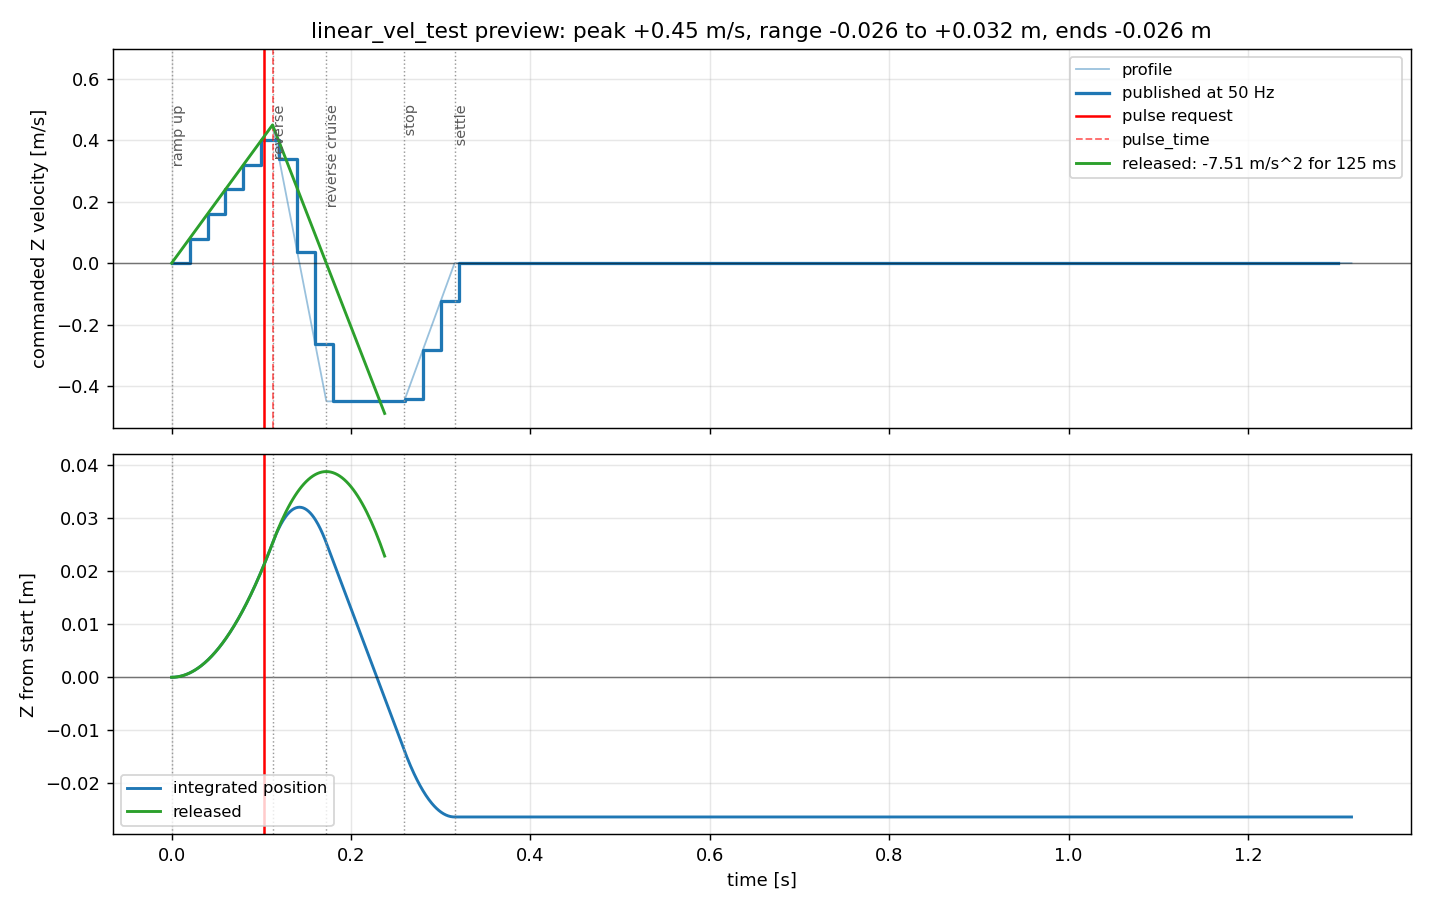
\includegraphics[width=0.92\linewidth]{figs/preview_linear_vel.png}
\caption{Output of \code{preview\_linear\_vel.py} with its defaults, generated by the script itself. Top:
commanded velocity, the \SI{50}{Hz} staircase actually published, and the released bar (green). Bottom:
integrated positions.}
\label{fig:preview}
\end{figure}

The preview draws hand and bar in the world frame. The regrasp depends only on their \emph{difference}. The rest
of this note works in the hand frame.

%==========================================================================
\section{Kinematics of a release, seen from the hand}
%==========================================================================
\subsection{Definitions}
Let $s$ be position along the fixed grasp axis, positive up the axis. The hand moves with $v_h(t)$ and
$a_h(t)=\dot v_h$. The gripper releases the bar at $t_r$ and re-grips it at $t_r+T_p$, where $T_p$ is the
effective open time. Relative quantities are bar minus hand:
\begin{equation}
w(t)=v_o(t)-v_h(t),\qquad \Delta(t)=\int_{t_r}^{t} w\,\mathrm d\tau ,\qquad w(t_r)=\Delta(t_r)=0 .
\end{equation}
$\Delta>0$ means the bar has moved up the hand, which is the \code{cuboid\_rel\_z} that the policy is rewarded
for. The quantities that matter are the slip at re-grip, $\Delta(t_r+T_p)$, and the relative speed at re-grip,
$w(t_r+T_p)$.

\subsection{Free bar (the preview's model)}
If only the axial gravity $g_a=g\cos\theta$ acts on the released bar, then
\begin{equation}
\dot w=-g_a-a_h(t).\label{eq:free}
\end{equation}
Take the preview's case: the release happens at the start of a reversal from $+v_0$ to $-v_1$ at constant
deceleration $A$, taking $T_r=V/A$ with swing $V=v_0+v_1$, followed by a cruise at $-v_1$. For
$T_p\ge T_r$, integrating \eqref{eq:free} gives (Appendix~\ref{app:derivation})
\begin{align}
w(T_p)&=V-g_aT_p, \label{eq:wend}\\
\Delta(T_p)&=V\,T_p-\frac{V^2}{2A}-\frac12 g_a T_p^2 . \label{eq:slip}
\end{align}
The relative motion peaks where $w=0$. A re-grip at that apex gives the largest slip, zero impact speed, and
first-order insensitivity to the pulse length, since $\partial\Delta/\partial T_p=w(T_p)$. The \emph{matched}
swing and the slip it produces are
\begin{equation}
V^{*}=g_aT_p\quad\Longleftrightarrow\quad v^{*}=\tfrac12 g_aT_p\ \ (v_0=v_1),\qquad
\Delta^{*}=\tfrac12 g_aT_p^2\Bigl(1-\frac{g_a}{A}\Bigr). \label{eq:match}
\end{equation}
Release timing matters much more. Differentiating \eqref{eq:slip}'s general form with respect to $t_r$ gives
\begin{equation}
\frac{\partial\Delta}{\partial t_r}=w(t_r+T_p)+T_p\bigl(a_h(t_r)+g_a\bigr).\label{eq:sens}
\end{equation}
The second term has no counterpart in $\partial\Delta/\partial T_p$. The hand's acceleration jumps at the
reversal, so $\Delta(t_r)$ has a kink there with slopes of opposite sign, and the maximum sits on the kink.

\paragraph{Numbers for the defaults.} $V=\SI{0.9}{m/s}$, $A=\SI{15}{m/s^2}$, $T_p=\SI{125}{ms}$ and
$g_a=\SI{7.51}{m/s^2}$ give $\Delta=\SI{26.8}{mm}$ and $w=\SI{-0.039}{m/s}$. The matched peak speed is
$v^*=\SI{0.470}{m/s}$ and $\Delta^*=\SI{29.3}{mm}$. \textbf{In the preview's own model, \SI{0.45}{m/s} is
matched at $40^\circ$.} The timing slopes are $+\SI{1.40}{mm/ms}$ for a release before the reversal (where
$a_h=+\SI{4}{m/s^2}$) and $\SI{-0.98}{mm/ms}$ for a release after it.

\subsection{The bar rests on the lower finger}
In the tilted posture the gravity component normal to the axis, $g_n=g\sin\theta$, does not point at empty
space. Rotating world gravity into the task frame of \code{env\_franka\_parallel\_tilted.py} at $40^\circ$ gives
$(-0.49,\,6.29,\,-7.51)\,\si{m/s^2}$. The transverse part is anti-parallel to the finger-closing axis
(cosine $-0.997$). So when the fingers open, the bar lies on the lower finger with normal load $m g_n$ and slides
against Coulomb friction $\mu m g_n$ (Figure~2 of the companion RL report). The relative dynamics become
piecewise:
\begin{equation}
\dot w=\begin{cases}
-\gp-a_h, & w>0\ \text{(sliding up)},\qquad \gp=g(\cos\theta+\mu\sin\theta),\\
-\gm-a_h, & w<0\ \text{(sliding down)},\qquad \gm=g(\cos\theta-\mu\sin\theta),\\
0, & w=0\ \text{and}\ |g_a+a_h|\le \mu g_n\ \text{(stuck)}.
\end{cases}\label{eq:coulomb}
\end{equation}
Three consequences follow for $\theta=40^\circ$ and $\mu=0.75$, where $\gp=\SI{12.24}{m/s^2}$ and
$\gm=\SI{2.79}{m/s^2}$:
\begin{enumerate}
\item \textbf{Up-slip needs $A>\gp$.} The bar moves up the hand only while the hand decelerates faster than
\SI{12.2}{m/s^2}. The commanded \SI{15}{m/s^2} leaves a margin of \SI{2.8}{m/s^2}, against \SI{7.5}{m/s^2} in the
free model.
\item \textbf{The apex comes early and the rest of the pulse is spent sliding back.} Replacing $g_a$ by $\gp$ in
\eqref{eq:match} gives $v^*=\tfrac12\gp T_p=\SI{0.765}{m/s}$ for \SI{125}{ms}. Equivalently, the matched pulse
for $v=\SI{0.45}{m/s}$ is $T^*=2v/\gp=\SI{73.5}{ms}$. After the apex the bar slides down at $\gm$. It sticks only
if $\tan\theta\ge1/\mu$, i.e.\ $\theta\ge53^\circ$ for $\mu=0.75$.
\item \textbf{$v^*$ is almost independent of tilt.} $\cos\theta+\mu\sin\theta$ peaks at $\theta=\arctan\mu$,
where $v^*=\tfrac12 gT_p\sqrt{1+\mu^2}$ (\SI{0.77}{m/s} for $\mu=0.75$). At $0^\circ$ it is
$\tfrac12 gT_p=\SI{0.61}{m/s}$. For every tilt from $0^\circ$ to $45^\circ$ and $\mu\ge0.5$, a \SI{125}{ms}
pulse needs \SIrange{0.61}{0.87}{m/s} (Figure~\ref{fig:matched}).
\end{enumerate}

\begin{figure}[t]
\centering
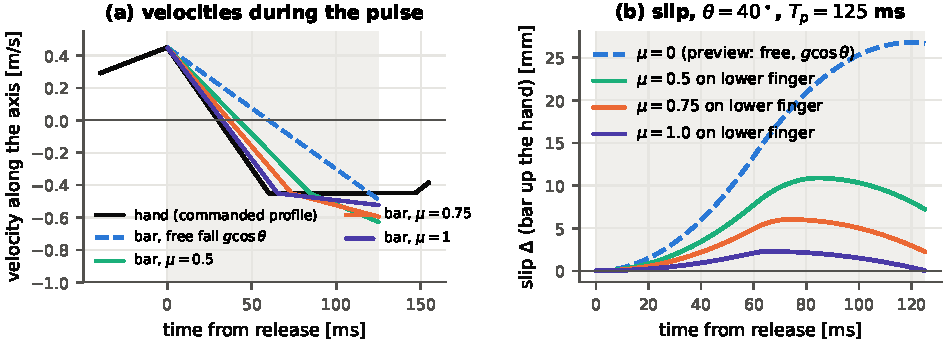
\includegraphics[width=\linewidth]{figs/relative_view.pdf}
\caption{The preview's profile in the hand frame, using the idealized hand (the commanded profile itself) and a
release at the reversal. (a) Velocities: the free-fall bar (dashed) reaches the hand's cruise speed only at the
end of the pulse, while the bar sliding on the lower finger gets there after \SIrange{65}{85}{ms}. (b) Slip.
Without friction the re-grip catches the bar at its apex (\SI{26.8}{mm}). With $\mu=0.75$ the apex is
\SI{6.0}{mm} at \SI{74}{ms}, and \SI{2.3}{mm} is left at re-grip.}
\label{fig:relview}
\end{figure}

\begin{figure}[t]
\centering
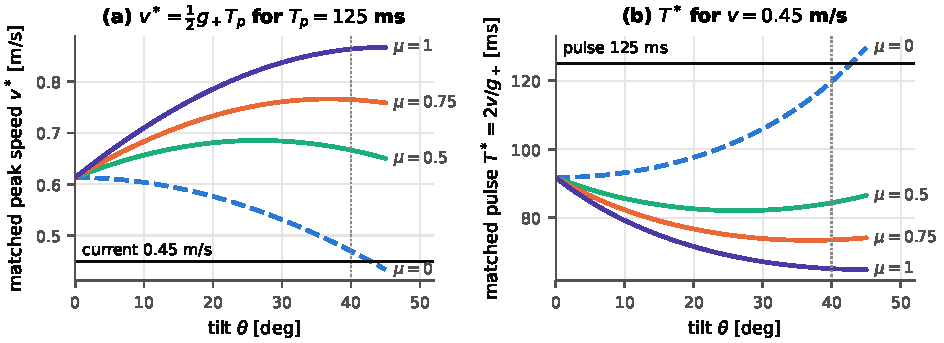
\includegraphics[width=\linewidth]{figs/matched.pdf}
\caption{(a) Matched peak speed for a \SI{125}{ms} pulse versus tilt, from Eq.~\eqref{eq:match} with $g_a$
replaced by $\gp$. The dashed curve is the preview's frictionless model: it crosses \SI{0.45}{m/s} only near
$40^\circ$, the tilt the preview uses. (b) Matched open time for $v=\SI{0.45}{m/s}$.}
\label{fig:matched}
\end{figure}

%==========================================================================
\section{Validation in Genesis}
%==========================================================================
\label{sec:validation}
The model was checked against the simulator the policy was trained in. Two tools were added under
\code{reports/tools/}.
\begin{itemize}
\item \code{pulse\_slip\_sweep.py} drives \code{env\_franka\_parallel\_tilted.py} with the same profile shape as
\code{linear\_vel\_test.py}: ramp at \SI{4}{m/s^2}, reverse at \SI{15}{m/s^2}, cruise, stop. It fires one
pulse per environment. Each environment has its own peak speed, pulse length $L$ (forced-open window
$(L-1)\times\SI{20}{ms}$) and trigger offset. Finger gain ($k_p=300$) and friction are pinned, and the pulse
delay is set to zero so the forced-open window starts at the trigger.
\item \code{pulse\_hires.py} wraps \code{scene.step} to log hand velocity, bar velocity, in-hand position and
finger contact force at \SI{1}{kHz}, for five friction values. It also measures the angle between the transverse
gravity and the finger axis.
\end{itemize}

\paragraph{Release timing is what friction changes at $0^\circ$.} At zero tilt the bar is free once released.
Yet the slip at a fixed profile went from \SI{-4.0}{mm} ($\mu=0.25$) through \SI{1.3}{mm} and \SI{12.2}{mm} to
\SI{21.0}{mm} ($\mu=1.0$). The contact force shows why. The residual squeeze carries the bar for a
$\mu$-dependent time after the trigger. Extrapolating the bar's free-flight line back to the hand velocity gives
an equivalent release instant of 0, 3, 11 and \SI{24}{ms}. Feeding those instants and Genesis' own hand velocity
into Eq.~\eqref{eq:free} reproduces the four slips within \SI{0.3}{mm} (Figure~\ref{fig:validation}a). This is
Eq.~\eqref{eq:sens} observed directly: \SI{24}{ms} of release delay is worth \SI{25}{mm} of slip. The optimum lies
where the hand actually starts to decelerate, about \SI{25}{ms} after the commanded reversal.

\paragraph{Friction on the lower finger at $40^\circ$ and $45^\circ$.} With the same release instants, the
Coulomb model \eqref{eq:coulomb} with the simulator's $\mu$ gives \SI{11.4}{mm} (Genesis \SI{11.3}{mm}) at $40^\circ$
and \SI{12.0}{mm} (Genesis \SI{12.2}{mm}) at $45^\circ$ for $\mu=0.75$. The free-fall model predicts \SI{26.3}{mm}
and \SI{29.3}{mm}. Across $\mu\in[0.25,1]$ the Coulomb model stays within \SI{3}{mm}, while the free model is off
by up to a factor of four and has the wrong trend: it predicts more slip for more friction
(Figure~\ref{fig:validation}b). Figure~5 of the companion RL report overlays the full \SI{1}{kHz} trace.

\begin{figure}[t]
\centering
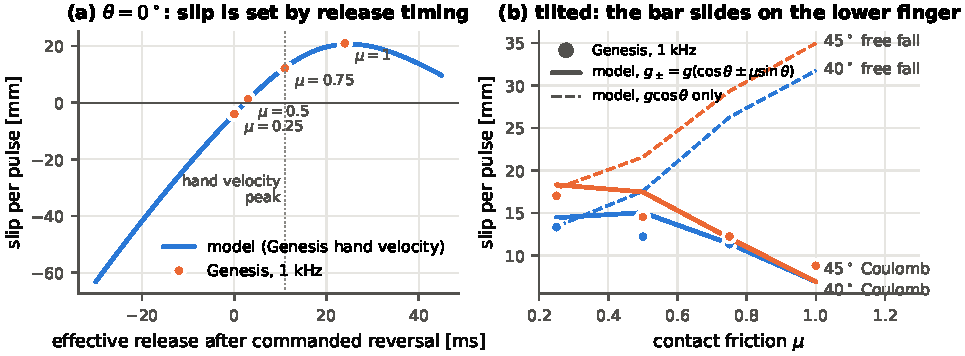
\includegraphics[width=\linewidth]{figs/validation.pdf}
\caption{Model versus Genesis at \SI{1}{kHz}, $v=\SI{0.45}{m/s}$, \SI{120}{ms} forced-open window. (a) At
$0^\circ$ the only effect of contact friction is to delay the effective release. The curve is
Eq.~\eqref{eq:free} evaluated with Genesis' hand velocity. (b) At $40^\circ$ and $45^\circ$ the free-fall model
(dashed) fails. The Coulomb model \eqref{eq:coulomb} (solid) matches.}
\label{fig:validation}
\end{figure}

\paragraph{Velocity against pulse length.} Figure~\ref{fig:gensweep} sweeps peak speed and open window in
Genesis, with the trigger at the commanded reversal. At $40^\circ$ and \SI{0.45}{m/s} the slip peaks at a
\SI{100}{ms} window (\SI{12.0}{mm}) and falls to 11.3, 8.9 and \SI{6.1}{mm} at 120, 140 and \SI{160}{ms}: the
pulse outlasts the apex. At \SI{0.65}{m/s} the slip rises to 23.6, 24.7 and \SI{24.4}{mm}, a plateau that no longer
depends on pulse length. That is the matched condition, reached at the speed Figure~\ref{fig:matched} predicts.
At $0^\circ$, with no friction to slow the back-slide, \SI{0.45}{m/s} collapses from \SI{13.1}{mm} to
\SI{-5.1}{mm} over the same windows.

\begin{figure}[t]
\centering
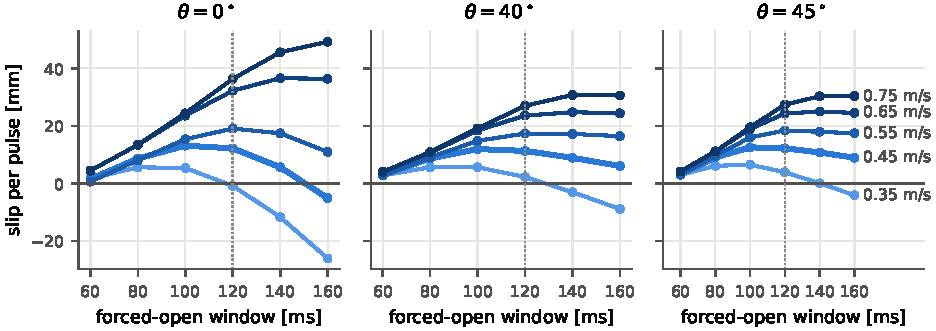
\includegraphics[width=\linewidth]{figs/genesis_velocity_sweep.pdf}
\caption{Genesis: slip per pulse against the forced-open window, for peak speeds from 0.35 to \SI{0.75}{m/s}
(the thick line is \SI{0.45}{m/s}). The dotted line marks the \SI{120}{ms} window of the current environment.
Curves that fall after their peak belong to pulses longer than the apex. Flat tops are matched.}
\label{fig:gensweep}
\end{figure}

%==========================================================================
\section{What the arm actually does}
%==========================================================================
\subsection{The reference chain}
The controller does not play the profile. It plays what reaches it, and the default configuration
(\code{config/cartesian\_velocity\_torque.yaml}) reshapes that in four stages:
\begin{enumerate}
\item \textbf{Publishing at \SI{50}{Hz}.} The profile reverses at \SI{112.5}{ms}, between the ticks at 100 and
\SI{120}{ms}. The published staircase goes $0.40\to0.34$ and \textbf{never contains \SI{0.45}{m/s}}.
\item \textbf{\code{interp: cubic}, \code{interp\_lag: 1.0}.} This plays the segment that ends at the newest
command, which is one \code{command\_period} (\SI{20}{ms}) late by construction.
\item \textbf{Low-pass} ($\omega_n=\SI{400}{rad/s}$, $\zeta=0.61$; about \SI{3}{ms} of delay) and the
\code{max\_accel}\,$=\SI{19}{m/s^2}$ slew limit.
\item \textbf{The arm's own tracking.} This is modelled with the 2nd-order filter the Genesis environment uses
as its stand-in ($\omega_n=\SI{75}{rad/s}$, $\zeta=0.33$, tuned against the real arm).
\end{enumerate}
With the defaults, the modelled hand peaks at \SI{0.405}{m/s} and dips to \SI{-0.55}{m/s}. Its actual reversal
comes \SI{28}{ms} after the commanded one and \SI{38}{ms} after the pulse request (Figure~\ref{fig:chain}). The
preview's green curve starts at \SI{0.45}{m/s}, \SI{0.045}{m/s} faster than the hand. Over a \SI{125}{ms}
pulse that difference alone is worth about \SI{5.6}{mm} of slip.

\begin{figure}[t]
\centering
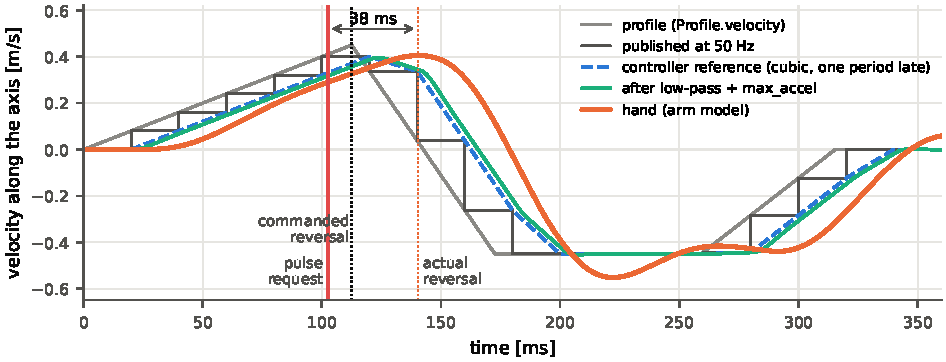
\includegraphics[width=\linewidth]{figs/chain.pdf}
\caption{From \code{Profile.velocity} to the hand, stage by stage. The request goes out \SI{10}{ms} before the
commanded reversal. The hand reverses \SI{38}{ms} after the request.}
\label{fig:chain}
\end{figure}

\subsection{Timing budget}
The release happens at
\begin{equation}
t_r=t_{\text{rev}}^{\text{cmd}}-t_{\text{lead}}+L_g ,
\end{equation}
where $L_g$ is the Robotiq's latency from service request to the bar coming loose. It has not been measured; the
README asks for that measurement before a lead is chosen. Slip is largest when $t_r$ falls on or slightly after
the \emph{actual} reversal, so the lead should be
\begin{equation}
t_{\text{lead}}\approx L_g-\tau_{\text{chain}},\qquad \tau_{\text{chain}}\approx\SI{28}{ms}.
\end{equation}
Figure~\ref{fig:latency} shows slip as a function of $L_g$ for the current \SI{10}{ms} lead. With the defaults
and $\mu=0.75$, the best case is only \SI{4.7}{mm} (at $L_g\approx\SI{26}{ms}$), and the bar is sliding down at
\SI{0.17}{m/s} when caught. The preview's free-fall model predicts \SI{23.5}{mm} under the same chain.

\begin{figure}[t]
\centering
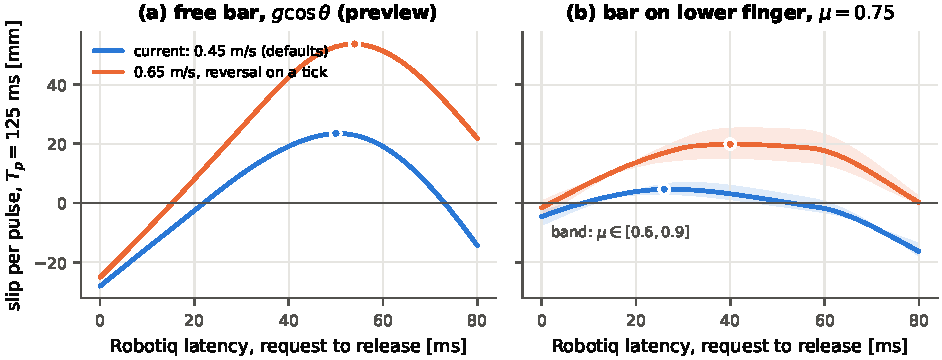
\includegraphics[width=\linewidth]{figs/latency.pdf}
\caption{Slip for a \SI{125}{ms} pulse at $40^\circ$ against Robotiq latency, with the current \SI{10}{ms} lead
and the modelled hand from Figure~\ref{fig:chain}. (a) Free bar. (b) Bar on the lower finger, with the band
covering $\mu\in[0.6,0.9]$. Dots mark the best latency. At \SI{0.65}{m/s} the curve in (b) is flat within
\SI{1}{mm} over $\pm\SI{10}{ms}$ of latency.}
\label{fig:latency}
\end{figure}

%==========================================================================
\section{Why 0.45 m/s is not the right speed for this pulse}
%==========================================================================
The four problems are:
\begin{enumerate}
\item \textbf{The match in the preview is a coincidence of its assumptions.} Without friction, \SI{0.45}{m/s} is
matched only near $40^\circ$ (Figure~\ref{fig:matched}a, dashed curve). At $0^\circ$ the frictionless $v^*$ is
already \SI{0.61}{m/s}.
\item \textbf{With the bar on the lower finger, a \SI{125}{ms} pulse outlasts the apex by about \SI{50}{ms}.} The
end of the pulse gives slip back, so the fingers close on a bar moving down at \SIrange{0.15}{0.2}{m/s}. The
result then depends on the pulse length itself, since $\partial\Delta/\partial T_p=w\approx\SI{-0.17}{m/s}$, or
\SI{1.7}{mm} per \SI{10}{ms}. Genesis shows the same thing (Figure~\ref{fig:gensweep}).
\item \textbf{The arm never reaches \SI{0.45}{m/s}.} The reversal falls between publish ticks, and the hand
reverses \SI{28}{ms} late.
\item \textbf{A pulse that outlasts the apex is sensitive to everything.} Figure~\ref{fig:design} maps slip and
``slip lost after the apex'' over peak speed and pulse length. The current point sits well inside the region
where part of the pulse is wasted. The black line ($w=0$ at re-grip) crosses $T_p=\SI{125}{ms}$ at about
\SI{0.70}{m/s} (\SI{23}{mm} of slip). At \SI{0.45}{m/s} the apex is reached with an \SI{85}{ms} pulse
(\SI{11.5}{mm}).
\end{enumerate}

\paragraph{Peak speed across tilts.} Figure~\ref{fig:tiltsweep} keeps the current pulse and sweeps the peak
speed for $\theta=0^\circ,10^\circ,\dots,45^\circ$. At \SI{0.45}{m/s} the slip barely depends on tilt:
\SIrange{4.6}{7.6}{mm} in the model and \SIrange{9.9}{12.2}{mm} in Genesis. The reason is that friction and
axial gravity trade off: a larger tilt lowers $g\cos\theta$ but raises the friction $\mu g\sin\theta$ on the
lower finger. Below about \SI{0.4}{m/s} the throw loses ground, and the bar ends \emph{lower} in the hand, most
of all at small tilts, where nothing holds it during the back-slide. The matched speed, marked with dots, rises
from \SI{0.62}{m/s} at $0^\circ$ to \SIrange{0.69}{0.70}{m/s} at $30^\circ$--$45^\circ$, and gives
\SIrange{23}{26}{mm} of slip. Genesis rises steadily up to the largest speed tested: \SI{36}{mm} at $0^\circ$
and \SIrange{27}{28}{mm} at $30^\circ$--$45^\circ$ at \SI{0.75}{m/s}, with no environment resets anywhere in
the sweep. In both panels \SI{0.45}{m/s} sits on the steep, shallow-slip part of every curve.

\begin{figure}[t]
\centering
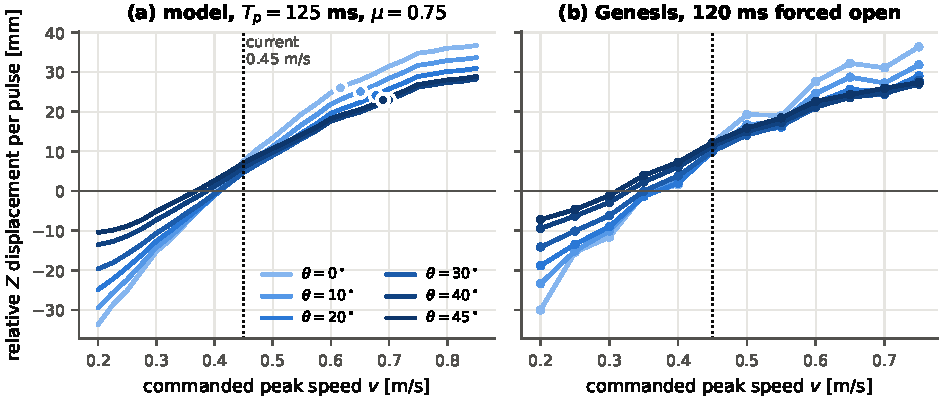
\includegraphics[width=\linewidth]{figs/tilt_velocity_sweep.pdf}
\caption{Relative $Z$ displacement (slip up the hand) per pulse against commanded peak speed, for tilts from
$0^\circ$ to $45^\circ$. (a) Model through the full controller chain, $T_p=\SI{125}{ms}$, $\mu=0.75$, reversal on
a publish tick, release on the hand's actual reversal. Dots mark the matched speed ($w=0$ at re-grip).
(b) Genesis, scripted throws with a \SI{120}{ms} forced-open window, trigger at the commanded reversal.}
\label{fig:tiltsweep}
\end{figure}

\paragraph{Friction sweep.} The real value of $\mu$ between bar and Robotiq pads is unknown, so
Figure~\ref{fig:fricsweep} and Table~\ref{tab:vstar} repeat the matched-speed calculation for
$\mu\in[0,1]$ at each tilt. The closed form is
\begin{equation}
v^*(\theta,\mu)=\tfrac12\,g\,T_p\,(\cos\theta+\mu\sin\theta).
\end{equation}
It equals the vertical value $\tfrac12 gT_p=\SI{0.61}{m/s}$ exactly when $\mu=\tan(\theta/2)$ (0.41 at
$45^\circ$). Below that friction the tilted grasp needs a slower throw than the vertical one; above it, a faster
one. The full-chain values follow the same pattern with a flatter slope, because the hand's overshoot enlarges the
real swing. At $\mu=0.3$ the matched speed is \SIrange{0.55}{0.63}{m/s} for every tilt. The only corner where
\SI{0.45}{m/s} comes close is a nearly frictionless bar at $40^\circ$--$45^\circ$ ($v^*=0.46$--\SI{0.49}{m/s}
at $\mu=0$). That is the preview's assumption. The slip at $v^*$ (Figure~\ref{fig:fricsweep}b) falls with
friction at large tilts, from about \SI{31}{mm} at $\mu\le0.3$ to \SI{17}{mm} at $\mu=1$ for $45^\circ$. At
$0^\circ$ it is independent of $\mu$, since there is no normal load.

\begin{figure}[t]
\centering
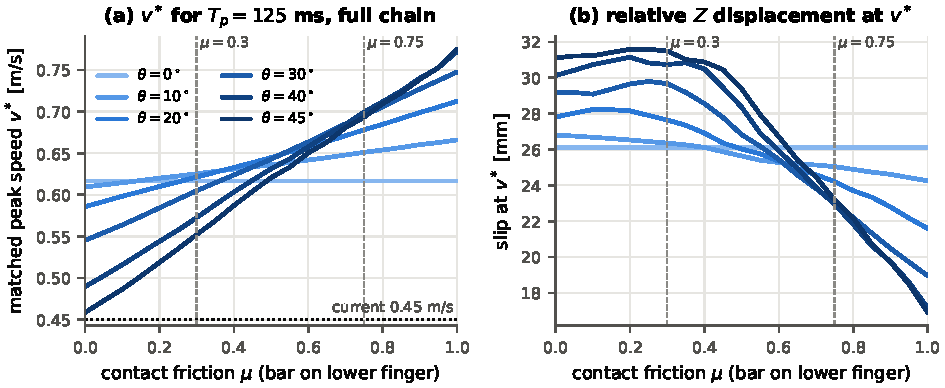
\includegraphics[width=\linewidth]{figs/friction_sweep.pdf}
\caption{Matched peak speed (a) and the slip it produces (b) against the friction between the bar and the lower
finger, one curve per tilt. Full controller chain, $T_p=\SI{125}{ms}$, reversal on a publish tick, release on the
hand's actual reversal. At $0^\circ$ friction has no effect.}
\label{fig:fricsweep}
\end{figure}

\begin{table}[h]
\centering\small
\caption{Matched peak speed $v^*$ [m/s] for $T_p=\SI{125}{ms}$: closed form $\tfrac12gT_p(\cos\theta+\mu\sin\theta)$
/ full controller chain.}
\label{tab:vstar}
\begin{tabular}{lccccc}
\toprule
tilt & $\mu=0$ & $\mu=0.3$ & $\mu=0.5$ & $\mu=0.75$ & $\mu=1.0$\\
\midrule
\csname @@input\endcsname friction_table.tex
\bottomrule
\end{tabular}
\end{table}

\begin{figure}[t]
\centering
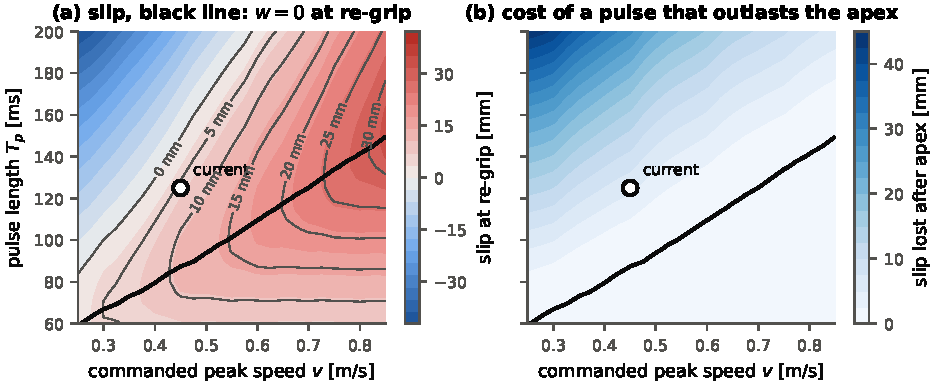
\includegraphics[width=\linewidth]{figs/design_map.pdf}
\caption{Design map at $40^\circ$ and $\mu=0.75$, with the modelled hand and the release on its actual reversal.
(a) Slip at re-grip. (b) Slip lost between the apex and the re-grip. The black line is the matched condition
$w(T_p)=0$. Points below it re-grip before the apex, points above it after.}
\label{fig:design}
\end{figure}

\begin{table}[h]
\centering\small
\caption{Four profiles through the full chain, $\theta=40^\circ$, $\mu=0.75$, with the lead set to each profile's
best latency. ``Tick'' means \code{accel\_up} chosen so that the reversal falls on a publish tick
($v/a_{\text{up}}$ a multiple of \SI{20}{ms}). Columns: slip at best latency; slip at $\pm\SI{10}{ms}$ of latency
error; slip for $\mu\in[0.6,0.9]$; relative speed at re-grip; free-fall slip at its own best latency (the
preview's model); modelled hand peak/trough; commanded travel above/below the start.}
\label{tab:design}
\setlength{\tabcolsep}{3.5pt}
\begin{tabular}{lcccccccccc}
\toprule
profile & $v$ & $T_p$ & $L_g^{\text{best}}$ & slip & $\pm$10 ms & $\mu$ band & $w$ & free & hand & travel\\
 & [m/s] & [ms] & [ms] & [mm] & [mm] & [mm] & [m/s] & [mm] & [m/s] & [mm]\\
\midrule
\csname @@input\endcsname design_table.tex
\bottomrule
\end{tabular}
\end{table}

%==========================================================================
\section{Recommendations}
%==========================================================================
\begin{enumerate}
\item \textbf{Match the speed to the pulse, not the other way round, when the pulse is fixed by the gripper.}
For $T_p\approx\SI{125}{ms}$ use about \SI{0.65}{m/s}, for example
\begin{center}\code{target\_vel:=0.65\ \ accel\_up:=3.6111\ \ reverse\_hold:=0.15}\end{center}
which puts the reversal on the \SI{180}{ms} tick. The model gives
\SI{19.9}{mm} per pulse at zero relative speed, holding within \SI{1}{mm} over $\pm\SI{10}{ms}$ of latency.
Genesis gives \SIrange{23.6}{24.7}{mm}, flat in pulse length. The costs are more travel ($+73/-68$ mm, within
\code{max\_travel}\,$=\SI{0.3}{m}$) and hand speeds up to \SI{0.71}{m/s}, below \code{max\_velocity}. The trained
policy is capped at \SI{0.45}{m/s} (\code{Z\_VEL\_MAX}), so for closed-loop use it would need retraining with a
higher cap.
\item \textbf{Or keep \SI{0.45}{m/s} and shorten the effective open time to about \SI{85}{ms}.} The model gives
\SI{11.6}{mm} per pulse at zero relative speed, holding within \SI{1.4}{mm} over $\pm\SI{10}{ms}$. This suits
fine steps; the target range is 12.5 to \SI{22.5}{mm}.
\item \textbf{Put the reversal on a publish tick.} Choose $v/a_{\text{up}}$ as a multiple of \SI{20}{ms}. With
the defaults only the tick alignment changes, and the hand peak rises from 0.405 to \SI{0.44}{m/s} (slip 4.7 to
\SI{7.4}{mm}).
\item \textbf{Measure the gripper.} Record the request, the width feedback and the arm twist with
\code{plot\_velocity\_log.py} for ten pulses. That gives $L_g$ and its jitter, plus the effective open time
$T_p$. Then set $t_{\text{lead}}=L_g-\SI{28}{ms}$.
\item \textbf{Measure $\mu$ with the gripper open.} Tilt the open hand with the bar resting on the lower finger
until it stops sliding: $\mu=1/\tan\theta_{\text{stick}}$. Alternatively, fit $\mu$ from the slip of a few
pulses using Eq.~\eqref{eq:coulomb}, as done for Genesis in Section~\ref{sec:validation}.
\item \textbf{Extend the preview.} Two additions would make its green curve predictive: the $\mu g\sin\theta$
term, and the chain of Figure~\ref{fig:chain} applied to the hand. Both are about twenty lines, using
\code{controller\_chain} and \code{simulate\_slip} in \code{reports/tools/slip\_model.py}.
\end{enumerate}

\paragraph{Limitations.} The model is one-dimensional. It ignores bar rotation, finger compliance and the
opening and closing transients (Genesis shows these as the $\mu$-dependent release delay). The arm stage borrows
the Genesis stand-in instead of a measured real-arm response. The Genesis results use the Franka hand model, not
the Robotiq 2F. All of this points the same way: the numbers are best read as trends and orders of magnitude,
to be calibrated with the two measurements above.

\appendix
%==========================================================================
\section{Derivation of Eqs.~(\ref{eq:wend})--(\ref{eq:sens})}
\label{app:derivation}
%==========================================================================
Release at $\tau=0$ at hand speed $v_0$. The bar moves as $v_o(\tau)=v_0-g_a\tau$. The hand decelerates at $A$
until $T_r=V/A$ and then cruises at $-v_1=v_0-V$. For $\tau\ge T_r$:
\begin{align*}
\int_0^{T_p}v_o\,\mathrm d\tau&=v_0T_p-\tfrac12 g_aT_p^2,\\
\int_0^{T_p}v_h\,\mathrm d\tau&=v_0T_r-\tfrac12 A T_r^2-v_1(T_p-T_r)=\tfrac12(v_0-v_1)T_r-v_1(T_p-T_r),\\
\Delta&=\int_0^{T_p}(v_o-v_h)\,\mathrm d\tau=V\,T_p-\tfrac12 V T_r-\tfrac12 g_aT_p^2
=V\,T_p-\frac{V^2}{2A}-\tfrac12 g_aT_p^2 ,
\end{align*}
and $w(T_p)=v_0-g_aT_p-(-v_1)=V-g_aT_p$. Setting $w=0$ gives $V^*=g_aT_p$, and substituting it back gives
$\Delta^*=g_aT_p^2-\tfrac{g_a^2T_p^2}{2A}-\tfrac12g_aT_p^2=\tfrac12g_aT_p^2(1-g_a/A)$. For a general hand profile,
$\Delta(t_r)=\int_{t_r}^{t_r+T_p}\bigl[v_h(t_r)-g_a(t-t_r)-v_h(t)\bigr]\mathrm dt$. The Leibniz rule gives the
integrand at the upper limit, which is $w(t_r+T_p)$, minus the integrand at the lower limit, which is $0$, plus
$\int\partial_{t_r}[\cdot]=T_p(a_h(t_r)+g_a)$. That is Eq.~\eqref{eq:sens}. With friction, $g_a$ is replaced by
$\gp$ for as long as $w>0$.

%==========================================================================
\section{Reproduction}
%==========================================================================
\begin{verbatim}
# Genesis experiments (in the genesis container, workspace at /workspace)
python3 reports/tools/pulse_slip_sweep.py --tilts 0 15 30 45 \
        --out reports/data/pulse_slip.npz
python3 reports/tools/pulse_slip_sweep.py --tilts 0 40 45 \
        --vpeaks 0.35 0.45 0.55 0.65 0.75 --lengths 4 5 6 7 8 9 \
        --offsets -1 0 1 --zvel-max 0.8 --out reports/data/pulse_slip_fast.npz
python3 reports/tools/pulse_hires.py --tilts 0 40 45 \
        --out reports/data/pulse_hires.npz
# figures, table and numbers (host, no Genesis needed)
python3 reports/controller_pulse/make_figs.py
cd reports/controller_pulse && latexmk -pdf pulse_velocity_analysis.tex
\end{verbatim}
\code{make\_figs.py} writes every number quoted here to \code{numbers.json}, and the table rows to
\code{design\_table.tex}.

\end{document}
